%!TEX root = ../Master.tex
\chapter{Discussion}

In this chapter the program will be evaluated in context to what there should be improved upon in order to implement the program at a hospital complex. The program will also be looked at in relation to what it could be used for in other situations.

\section{Possible program improvements}

Consider the following situation; an user wants to find the fastest route from first floor to third floor. The user does not have any disabilities so both elevators and stairs can be part of the fastest route. The current program would most likely guide the user to the elevator from the first floor to the third floor. However it would be a problem if the elevator was already in use at the sixth floor. The user would then have to wait for the elevator to descent, this could take some time. If the program had the ability to track the location of the elevator, it could use this information in the algorithm of the program. The program would then have enough data to guide the user up the stairs, providing the user with a faster route. 
\newline
After the program have generated a route, it will keep the it until it is prompted to make a new one. An improvement to this would be if the program generated a new route if the user got of the route. This means if a hallway is blocked or in another way obstructed, the user will still be able to get to their destination. It should only calculate a new route if the user diverted too much from the original one, otherwise a little inaccuracy from the accelerometer would make the program calculate a new route without it being necessary. In order to implant this, the program should evaluate its coordinates after a specific number of seconds.
The program will be more useful for the visual impaired if it was able to give directions trough sound. This could be done by implementing Text to Speech \cite{diss_tss} and using it to read the directions the program outputs. If the program could receive audio commands such as "Direct me to the third floor, wing B" or "Take me to the nearest elevator" the visual impaired could use the program without using any visual clues.

\subsection{Implementation}

In order to have the final program, several sections of it have to be implemented. The program will need to receive positioning data and use it when calculating the route, as of now the user have to manually type in in where one is. The program needs a better method of communicating with the user, as of right now the program prints the vertices the route is split into. It would be more optimal if the user interaction where with more detailed text as "Go right at the next corridor". The user communication does not necessary have to go trough a text interface, a graphical interface similar to the one of GPS's would also be a good solution \cref{fig:TomTom}. The interface should as previous mentioned only be similar as some of the represented data on GPS will be unnecessary for users. This is information like speed and driving related information as parking lots etc. A graphical interface similar to TomTom would help the users to navigate, as visuals will give a better overview of the complex and the route. 

\begin{figure}
\centering
    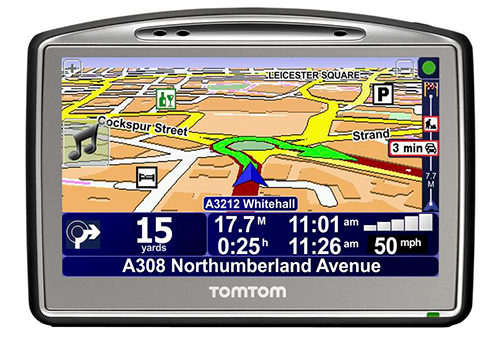
\includegraphics[width=\textwidth]{tomtom_go_720.jpg}
    \caption{A TomTom GPS \cite{diss_tomtom}.} \label{fig:TomTom}
\end{figure}


\section{Suggestions for Further Research}

The FLAWLESS algorithm is made to work in complexes. So far hospitals have been the focus of this project, but other complexes should be able to integrate this system as well. Such complexes could be shopping malls, ferries or exhibition halls. 

The shopping mall could benefit from this system as wheelchairs would be able to find elevators with more ease, and customers in general would easier find the various hops they are looking for. 

Exhibition halls are relevant to look at as s lot of people who have never been in these halls and could need help finding their way to the various booths. If the visitors could use the system to find their way to the booths they are looking for, less people would get lost and here would be less clutters of people as the times used on going from one pace to another will be reduced. 
\newline 

\section{External Factors}

A couple of observations that was made throughout the creation of this report considering the external factors, that can compromise the functionality of the program follows. The process of calibrating the graph in relation to the actual building, is considered to be paramount in order for the pathfinding algorithm to be able to find the optimal solution without failure. Because the algorithm removes all decision making from the user, the calculated route will always be optimal. There also lies a problem, in the implementation of the solution. If the users are not properly informed about the solution, they will not adapt it due to its foreign nature, and will continue using the status quo methods of navigation.